\textbf{COLUNI 2018 -- Questão 27}\par\medskip Uma senhora idosa, sentada em sua cadeira na sala e assistindo a um documentário sobre saúde e atividade física, assusta-se ao ouvir um forte barulho vindo da cozinha. Seu coração dispara imediatamente. Ela se pergunta: o que será que aconteceu? Tratava-se apenas de algumas louças que caíram da prateleira do armário.

\par

% COLUNI-AUTO-FIGURES-BEGIN
\begin{figure}[htbp]
\centering
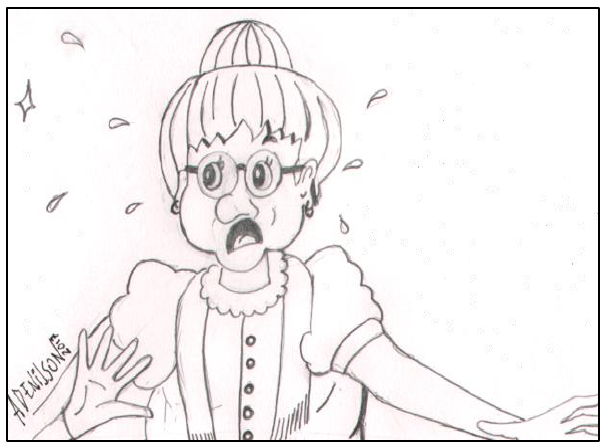
\includegraphics[width=0.95\linewidth]{static/simulados/coluni/figuras/2018/questao-27/figura-1.png}
\end{figure}
% COLUNI-AUTO-FIGURES-END

Após análise da situação e da figura acima e considerando como se dá a coordenação do organismo humano, é CORRETO afirmar que a senhora idosa:

\begin{enumerate}
\item recebeu a informação do ambiente externo por meio de órgão sensorial e a resposta, o susto, ocorreu
      pela coordenação do sistema nervoso e endócrino.
\item recebeu a informação do ambiente externo por meio de órgão sensorial e a resposta, o susto, ocorreu
      apenas pela coordenação do sistema nervoso.
\item recebeu a informação do ambiente interno por meio de órgão sensorial e a resposta, o susto, ocorreu pela
      coordenação do sistema nervoso e endócrino.
\item recebeu a informação do ambiente externo e interno por meio de órgão sensorial e a resposta, o susto,
      ocorreu apenas pela coordenação do sistema nervoso.\end{enumerate}
